\section{Introduction}
%Introduce veritesting, present our simple example and its performance improvement, segue into how veritesting at Java bytecode level is different from binary level
Symbolic execution is a popular testing technique that performs non-standard execution of a program.
%
Having been originally proposed in the 1970s, it has been applied for test generation~\cite{dart,cute}, equivalence checking~\cite{ramos,adaptorsynth}, finding vulnerabilities~\cite{driller,angr}, and even for checking correctness of transport protocols~\cite{transport}.
%
However, scalability continues to remain a challenge for symbolic execution.
%
Veritesting~\cite{veritesting} is a recently proposed technique that uses static symbolic execution to improve the scalability of dynamic symbolic execution.
%
It has been shown to find more bugs, and achieve more node and path coverage, when implemented at the X86 binary level.
%
This provides motivation for investigating integration of veritesting with symbolic execution at the Java bytecode level.

\lstinputlisting[caption={An example with a symbolic loop bound and nine execution paths through the loop body},
label={lst:v_ex}]{code_samples/VeritestingPerf.java}

Symbolic Pathfinder~(SPF)~\cite{spf} is a tool that performs symbolic execution of Java bytecode.
%
SPF is tightly integrated with Java PathFinder~(JPF)~\cite{jpf} and uses JPF extensions to replace concrete execution with symbolic execution.
%
We present an example demonstrating the potential benefit of integrating veritesting with SPF in Listing~\ref{lst:v_ex}.
%
The number of iterations done by the \textit{while} loop depends on the variable \textit{i}, which has been made symbolic.
%
The minimum and maximum values of symbolic integers is specified in a configuration file not shown here.
%
The presence of two three-way branches through the loop body creates nine execution paths.
%
Achieving complete path coverage when symbolically executing the \textit{while} loop beginning on line 9 requires a exponential number of paths with 9 as the base.
%
However, the three-way branches represent a comparison of \textit{x+i} with 0.
%
Such a comparison can be represented by SPF using the \textit{CMP} operator.
%
Each such three-way branch can be unrolled by using creating a symbolic formula as \textit{new BinaryNonLinearIntegerExpression(new BinaryNonLinearIntegerExpression(x\_v, PLUS, i\_v), CMP, new IntegerConstant(0))}.\mike{This looks weird because of the stupidity of the class names: there is nothing non-linear about what we are doing here.  It would be better with abstract names; in fact, it would be better still as the SMTLIB formula describing the region.  Could you replace w/the SMTLIB formula?}.

%
Statically unrolling the three-way branches from lines 11-16 creates a single execution path through the loop body.
%
Varying the range of symbolic integers in SPF from (-1, 1) to (-25, 25) using both, the plain and the statically unrolled symbolic formulas, causes the performance benefits of the latter version to be obvious.
%
We present such a comparison in Figure~\ref{fig:v_ex_plot}.\mike{This figure is ridiculously large vertically and we could use a little more space.  Shrink the scale and use numbers: 1, 10, 1000, ... as suggested by Stephen}
%
With the symbolic integer range being (-25, 25), plain SPF explores 7855 execution paths and takes 104 seconds on a Ubuntu 14.04 machine with Intel(R) Core(TM) i7-4790 and 16 GB RAM to achieve complete path coverage.
%
This is in contrast to SPF, summarizing the three-way branches with static unrolling, which explores 27 execution paths and takes a fraction of a second on the same machine to achieve complete path coverage.

\begin{figure}[]
\caption{Comparing number of execution paths from Listing~\ref{lst:v_ex} using vanilla SPF and SPF with static unrolling}
\label{fig:v_ex_plot}
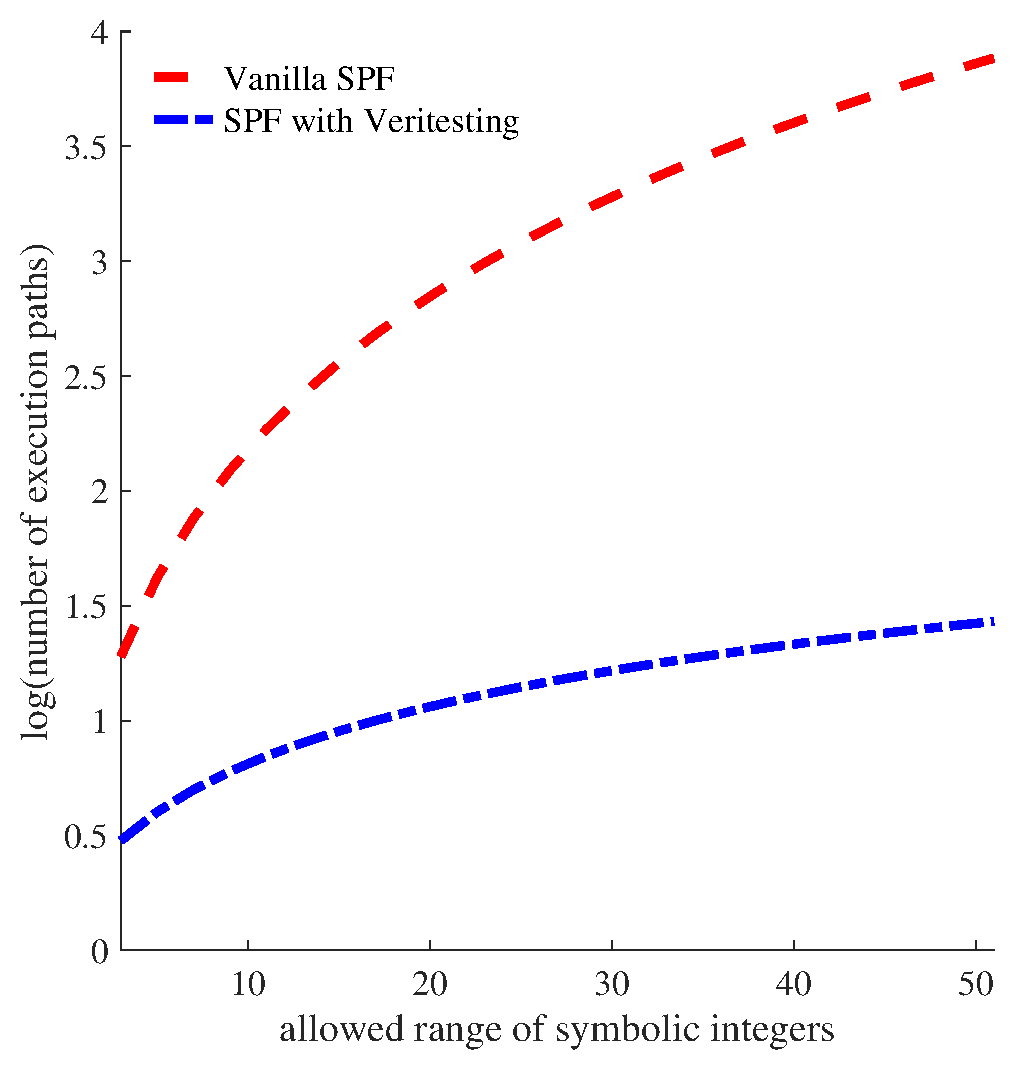
\includegraphics[width=\columnwidth]{figures/veritesting_example}
\end{figure}
%
